\begin{figure}
  \centering
  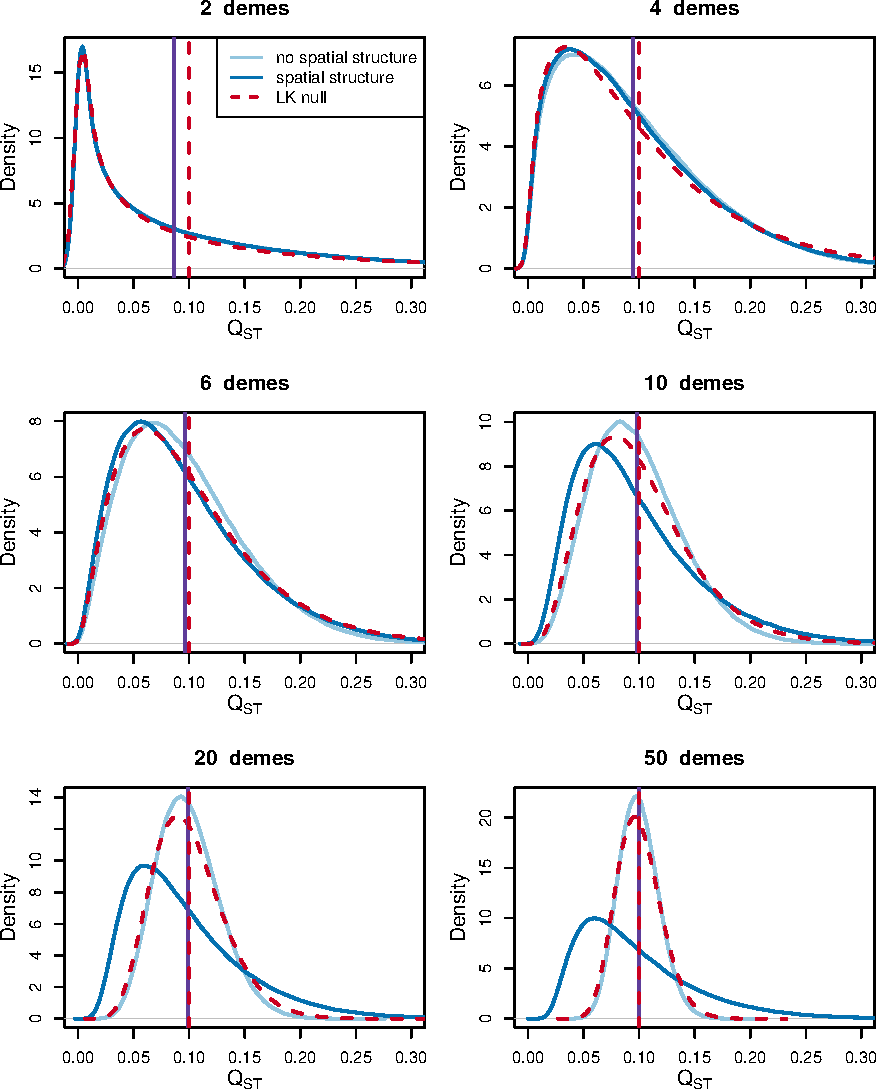
\includegraphics[width=0.8\textwidth]{figures/qst_deme_compare.pdf}
  \caption{\small The Lewontin-Krakauer (LK) distribution for $Q_{ST}$ is
    compared to the null distribution in the infinitesimal limit in a case with
    and a case without spatial structure. The case with no spatial structure
    assumes the migration rate is equal between all demes, and the case with
    spatial structure arranges demes in a ring with migration only between
    neighboring demes. Migration rates and subpopulation sizes are all equal and
    are set such that $F_{ST}=0.1$ even as the number of demes is increased
    \citep{Slatkin1991}. $Q_{ST}$ values for these models are simulated by
    drawing vectors from a multivariate normal distribution as described in the
    main text. In the LK distribution $Q_{ST}\sim F_{ST}\chi^2_{n_d -
      1}/(n_d-1)$, where $n_d$ is the number of demes. Vertical lines show the
    mean $Q_{ST}$ under the different null distributions. The mean $Q_{ST}$
    values for the two normal models are nearly identical. Discordance between
    these lines and that for the LK distribution illustrates that $Q_{ST} \neq
    F_{ST}$.}
  \label{fig:qst_deme}
\end{figure}
\begin{figure}
  \centering
  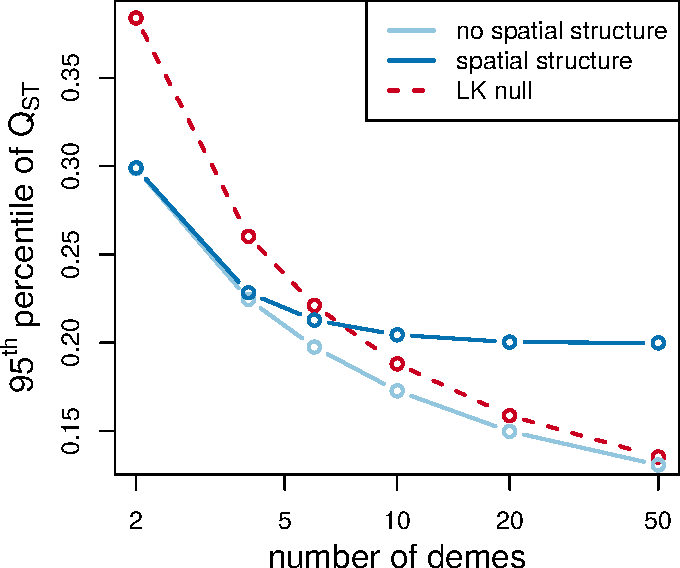
\includegraphics[width=0.5\textwidth]{figures/qst_deme_percentile_nospace.pdf}
  \caption{\small Differences in the $95^{\mathrm{th}}$ percentile of different
    $Q_{ST}$ null distributions. The Lewontin-Krakauer (LK) distribution is
    compared to null distributions for structured populations with and without a
    spatial component using the normal model.}
  \label{fig:qst_perc}
\end{figure}

Due to the build up of linkage disequilibrium between alleles affecting the
trait, the divergence in trait values among different subpopulations in a
structured population is about as variable as the variance in allele frequencies
\citep{Rogers1983}. We can apply the neutral theory of quantitative traits
developed above to obtain a null distribution for the divergence between groups
in structured populations. In obtaining this null distribution we use the normal
model found in the infinitesimal limit. A common way to quantify the divergence
in trait value between groups is $Q_{ST}$, defined as the variance between the
group means divided by the total variance in the population. The normal model
does not provide an analytic form for the neutral distribution of $Q_{ST}$, but
it does provide an efficient way to sample from this distribution. The null
distribution we obtain through this informed approach performs better than a
more naive null distribution suggested by \citet{Whitlock2009}.

Since we use a haploid model, we define $Q_{ST} = \frac{V_{between}}{V_{between}
  + V_{within}}$, where
\begin{equation*}
  V_{between} = \frac{1}{K} \sum_i \left( \bar{Y}_i - \bar{Y} \right)^2
\end{equation*}
and
\begin{equation*}
  V_{within} = \frac{1}{\sum_k N_k} \sum_i \sum_j \left( Y_{i,j} - \bar{Y}_i \right)^2.
\end{equation*}
Here, $Y_{i,j}$ is the trait value of individual $j$ in population $a$.

In the normal model, all $Y_{i,j}$ are normally distributed. Therefore,
$\bar{Y}_{i} - \bar{Y}$ and $Y_{i,j} - \bar{Y}_i$ are also normally distributed.
When population sizes are large, individual deviations from population means are
nearly uncorrelated as are $V_{between}$ and $V_{within}$. $V_{within}$ is
nearly constant across evolutionary realizations and is equal to $\sum_k N_k
E[\mathcal{T}_{k,k}] / \sum_k N_k$ because the within population variances are
approximately uncorrelated and their variances are order $1/N_k$. While we do
not have an explicit form for the between group variance, we can simulate from
its distribution by drawing a vector of $\bar{Y}_{i} - \bar{Y}$ values from a
multivariate normal distribution with mean zero and covariance matrix with
elements between populations $a$ and $b$
\begin{equation}
  \Cov[\bar{Y}_{a} - \bar{Y}, \bar{Y}_{b} - \bar{Y}] =
  \sigma^2(\E[\mathcal{T}_{a,\cdot}] + \E[\mathcal{T}_{b,\cdot}] -
  \E[\mathcal{T}_{\cdot,\cdot}] - \E[\mathcal{T}_{a,b}]).
\end{equation}
To simulate $Q_{ST}$ values we do not need to know $\sigma^2$ because the scale
of the trait variance cancels in the $Q_{ST}$ ratio. Knowing expected coalescent
times within and between populations, perhaps measured in units of mutations, is
sufficient for simulation.

A classic result in evolutionary quantitative genetics is that $Q_{ST}=F_{ST}$
\citep{Whitlock1999}. $F_{ST}$, in this context, refers to a parameter of the
population. In particular, $F_{ST} = \frac{\bar{t} - \bar{t}_0}{\bar{t}}$, where
$\bar{t}$ is the expected coalescent time for two loci sampled at random from
the entire population and $\bar{t}_0$ is the expected coalescent time for two
loci sampled within a subpopulation \citep{Slatkin1991}. This value is constant
over realizations of the evolutionary process. $Q_{ST}$ for a particular trait
could refer to a state of the population or to an estimate of this state. As
shown above, $Q_{ST}$, as a state of the population, varies across evolutionary
realizations. Thus, there is no sense in which $Q_{ST}$ can be defined a
constant parameter in the way that $F_{ST}$ can be. The expectation of
$V_{between}$ is $\bar{t} - \bar{t}_0$, and the expectation of $V_{within}$ is
$\bar{t}_0$. $\frac{\E[V_{between}]}{\E[V_{between}] + \E[V_{within}]}$ is equal
to $F_{ST}$, but due to Jensen's inequality, the expectation of this ratio
($\E[Q_{ST}]$) is always less than $F_{ST}$.

The null distribution of $Q_{ST}$ derived here could be useful in testing
whether an observed value is unlikley under neutrality. Current goodness-of-fit
tests either compare $Q_{ST}$ to an empirical distribution of $F_{ST}$ values or
to a $\chi^2$ distribution. In the second case, an identical distribution to
that developed by \citet{Lewontin1973} is used as the null distribution for
$Q_{ST}$. The $\chi^2$ testing procedure was suggested by \citet{Whitlock2009}
and is implemented in the program \textit{QstFstComp} \citep{Gilbert2015}. The
Lewontin-Krakauer (LK) distribution assumes independence between demes and
provides a good approximation in populations without spatial structure (Figure
\ref{fig:qst_deme}). When demes are strongly correlated, such as in spatial
structured populations, the LK distribution is a very poor approximation. Even
when the distributions appear qualitatively similar, there are substantial
differences in tail probabilities (Figure \ref{fig:qst_perc}).

The infinitesimal null distribution described here is similar to the extension
of the Lewontin-Krakuer $F_{ST}$ test developed by \citet{Bonhomme2010} to
account for the correlation structure between subpopulations. The
\citet{Bonhomme2010} method treats allele frequencies as multivariate normal
with covariance matrix parameteried by coancestry coefficients.
\citet{Ovaskainen2011} use a normal model similar to that found in the
infinitesimal limit here, but the covariance matrix is also based on coancestry
coefficients. When phenotypic and genetic divergence is mostly driven by changes
in allele frequency, the coalescent and coancestry based models should be very
similar. However, the coalescent model is ultimately preferable since it is the
correct null model at any scale of population divergence in the infinitesimal
limit. When only allele frequency data are available, a coancestry model is the
only option, but it is still better to model shared ancestry between populations
than to use a single value of $F_{ST}$.
%%% Local Variables:
%%% TeX-master: "short_report.tex"
%%% End:
